\begin{savequote}[75mm]
Some Quote.
\qauthor{Quoteauthor Lastname}
\end{savequote}

%For an example of a full page figure, see Fig.~\ref{fig:myFullPageFigure}.

\chapter{Patch-based Perceptual World Model}
\label{Chap:WorldModel}
\todo[inline]{Brief Introduction to 3D Data Acquisition and Representation (from Simon Thesis)}

\newthought{There's something to be said} for having a good opening line. 
\section{Octree Adjacency Graph}
\label{subsec:Adjacency}
Adjacency is a key element of the proposed method, as it ensures that supervoxels do not flow across object boundaries which are disconnected in space. There are three definitions of adjacency in a voxelized 3D space; 6-,18-, or 26-adjacent. These share a face, faces or edges, and faces, edges, or vertices, respectively. In this work, whenever we refer to adjacent voxels, we are speaking of 26-adjacency. 

As a preliminary step, we construct the adjacency graph for the voxel-cloud. This can be done efficiently by searching the voxel kd-tree, as for a given voxel, the centers of all 26-adjacent voxels are contained within $\sqrt{3}*R_{voxel}$. ${R}_{voxel}$ specifies the voxel resolution which will be used for the segmentation (for clarity, we shall simply refer to discrete elements at this resolution as voxels). The adjacency graph thus constructed is used extensively throughout the rest of the algorithm.

\section{Spatial Cluster Seeding}
\label{subsec:Seeding}
The algorithm begins by selecting a number of seed points which will be used to initialize the supervoxels. In order to do this, we first divide the space into a voxelized grid with a chosen resolution ${R}_{seed}$, which is significantly higher than ${R}_{voxel}$. The effect of increasing the seed resolution ${R}_{seed}$ can be seen in Figure~\ref{fig:SegmentedDiffSeeds}. Initial candidates for seeding are chosen by selecting the voxel in the cloud nearest to the center of each occupied seeding voxel.    




Once we have candidates for seeding, we must filter out seeds caused by noise in the depth image. This means that we must remove seeds which are points isolated in space (which are likely due to noise), while leaving those which exist on surfaces. To do this, we establish a small search radius ${R}_{search}$ around each seed, and delete seeds which do not have at least as many voxels as would be occupied by a planar surface intersecting with half of the search volume (this is shown by the green plane in Figure~\ref{fig:SeedingDiagram}). Once filtered, we shift the remaining seeds to the connected voxel within the search volume which has the smallest gradient in the search volume. Gradient is computed as
\begin{equation} \label{eqn:Gradient}
\mathit{G}(i) = \sum_{k\in{V}_{adj}}{\frac{\parallel{V(i)-V(k)}\parallel{}_{CIELab}}{{N}_{adj}}};
\end{equation}
we use sum of distances in CIELAB space from neighboring voxels, requiring us to normalize the gradient measure by number of connected adjacent voxels ${N}_{adj}$. Figure~\ref{fig:SeedingDiagram} gives an overview of the different distances and parameters involved in seeding.

%------------------------------------------------------------------------
\begin{figure}[t]
\begin{center}
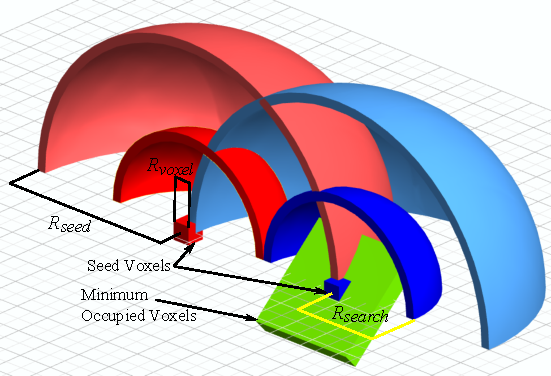
\includegraphics[width=0.9\linewidth]{figures/CVPR2013/MinimumOccupied.pdf}
\end{center}
   \caption[Seeding Parameters]{Seeding parameters and filtering criteria. ${R}_{seed}$ determines the distance between supervoxels, while ${R}_{voxel}$ determines the resolution to which the cloud is quantized. ${R}_{search}$ is used to determine if there are a sufficient number of occupied voxels to necessitate a seed. }
\label{fig:SeedingDiagram}
\end{figure}
%------------------------------------------------------------------------
%------------------------------------------------------------------------
\begin{figure*}
\begin{center}
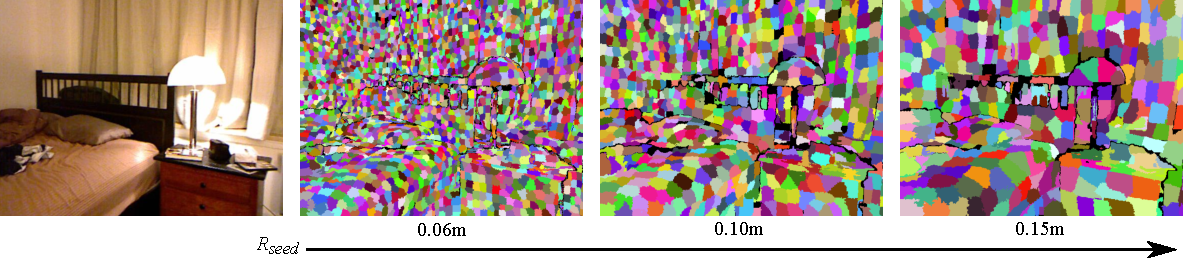
\includegraphics[width=1.0\linewidth]{figures/CVPR2013/IncreasingSeedSize.pdf}
\end{center}
   \caption[Seeding Size]{Image segmented using VCCS with seed resolutions of 0.1, 0.15 and 0.2 meters.}
\label{fig:SegmentedDiffSeeds}
\end{figure*}
%------------------------------------------------------------------------
Once the seed voxels have been selected, we initialize the supervoxel feature vector by finding the center (in feature space) of the seed voxel and connected neighbors within 2 voxels. 

\section{Cluster Features and Distance}
\label{subsec:Features}
VCCS supervoxels are clusters in a 39 dimensional space, given as 
\begin{equation}
\label{eqn:FeatureSpace}
\mathbf{F} = [x,y,z,L,a,b,\textrm{FPFH}_{1..33}],
\end{equation}
where $x,y,z$ are spatial coordinates, $L,a,b$ are color in CIELab space, and $\textrm{FPFH}_{1..33}$ are the 33 elements of Fast Point Feature Histograms (FPFH), a local geometrical feature proposed by Rusu et al.\@ \cite{FPFH}. FPFH are pose-invariant features which describe the local surface model properties of points using combinations of their \textit{k} nearest neighbors. They are an extension of the older Point Feature Histograms optimized for speed, and have a computational complexity of $O(n \cdot k)$.  

In order to calculate distances in this space, we must first normalize the spatial component, as distances, and thus their relative importance, will vary depending on the seed resolution ${R}_{seed}$. Similar to the work of Achanta et al.\@, \cite{SLICCompared} we have limited the search space for each cluster so that it ends at the neighboring cluster centers. This means that we can normalize our spatial distance $D_s$ using the maximally distant point considered for clustering, which will lie at a distance of $\sqrt{3} {R}_{seed}$. Color distance $D_c$, is the euclidean distance in CIELab space, normalized by a constant $m$. Distance in FPFH space, $D_f$, is calculated using the Histogram Intersection Kernel \cite{HistogramIntersection}. This leads us to a equation for normalized distance $D$:
\begin{equation}
\label{eqn:Distance}
D = \sqrt{\frac{\lambda D_c^2}{m^2}+\frac{\mu D_s^2}{3 {R}_{seed}^{2}}+\epsilon {D}_{HiK}^{2}},
\end{equation}
where $\lambda,\mu,$ and $\epsilon$ control the influence of color, spatial distance, and geometric similarity, respectively, in the clustering. In practice we keep the spatial distance constant relative to the other two so that supervoxels occupy a relatively spherical space, but this is not strictly necessary. For the experiments in this paper we have color weighted equally with geometric similarity.

\section{Flow Constrained Region Growing}
\label{subsec:FlowClustering}
Assigning voxels to supervoxels is done iteratively, using a local k-means clustering related to \cite{SLICCompared,DASP}, with the significant difference that we consider connectivity and flow when assigning pixels to a cluster. The general process is as follows: beginning at the voxel nearest the cluster center, we flow outward to adjacent voxels and compute the distance from each of these to the supervoxel center using Equation \ref{eqn:Distance}. If the distance is the smallest this voxel has seen, its label is set, and using the adjacency graph, we add its neighbors which are further from the center to our search queue for this label. We then proceed to the next supervoxel, so that each level outwards from the center is considered at the same time for all supervoxels. We proceed iteratively outwards until we have reached the edge of the search volume for each supervoxel (or have no more neighbors to check).

%------------------------------------------------------------------------
\begin{figure*}
\begin{center}
   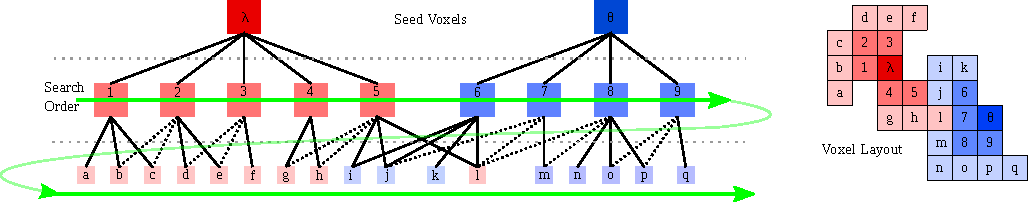
\includegraphics[width=0.95\linewidth]{figures/CVPR2013/SearchOrder.pdf}
\end{center}
   \caption[Voxel Search Order]{Search order for the flow constrained clustering algorithm (shown in 2D for clarity). Dotted edges in the adjacency graph are not searched, as the nodes have already been added to the search queue.}
\label{fig:ClusterSearch}
\end{figure*}
%------------------------------------------------------------------------


This amounts to a breadth-first search of the adjacency graph, where we check the same level for all supervoxels before we proceed down the graphs in depth. Importantly, we avoid edges to adjacent voxels which we have already checked this iteration. The search concludes for a supervoxel when we have reached all the leaf nodes of its adjacency graph or none of the nodes searched in the current level were set to its label. This search procedure, illustrated in Figure~\ref{fig:ClusterSearch}, has two important advantages over existing methods:

1. Supervoxel labels cannot cross over object boundaries that are not actually touching in 3D space, since we only consider adjacent voxels, and 

2. Supervoxel labels will tend to be continuous in 3D space, since labels flow outward from the center of each supervoxel, expanding in space at the same rate.

Once the search of all supervoxel adjacency graphs has concluded, we update the centers of each supervoxel cluster by taking the mean of all its constituents. This is done iteratively; either until the cluster centers stabilize, or for a fixed number of iterations. For this work we found that the supervoxels were stable within a few iterations, and so have simply used five iterations for all presented results. 

\section{Depth Adaptive Grid}
So far we have described the main algorithm for segmentation. Next we will introduce a generally applicable depth transform, which improves this specific analysis but can be used for all types of image analyses using algorithms with a fixed scale of observation on RGB-D data from a single RGB-D camera. In our case, we address shortcomings of the voxel grid VCCS is based on.

It is evident that observations from a single RGB-D camera have a significant drawback - the point density, and thus available detail of the scene geometry, falls rapidly with increasing distance from the camera. In addition, the levels of both quantization and noise grow quadratically \cite{ICCV11smisek, Khoshelham2012}, leading to a further degradation in the quality of geometric features. This change in point density with depth creates a tradeoff between capturing small-scale detail in the foreground (using small voxels) and avoiding noise in the background (using large voxels). This is a general problem which occurs in all algorithms working with a fixed scale (for example a radius search) on point clouds created from a single view.

We propose to compensate for the loss of point density and quantization with increasing depth $z$ by transforming the points into a skewed space using the transformation $T:(x,y,z)\rightarrow(x',y',z')$ with
      \begin{align}
    \begin{aligned}
    x'= x/z,~~~~y'= y/z,~~~~z' = \log(z)
    \end{aligned}
      \end{align}
The division of the $x$ and $y$ coordinates by $z$ reverses the perspective transformation, equalizing the point density in the $x$-$y$-plane. Transforming the $z$ coordinate helps to deal with the effects of depth quantization by compressing points as depth increases. It is easy to show that the transformation has the following property:
\begin{align}
  \frac{\partial x'}{\partial x} = \frac{\partial y'}{\partial y} = \frac{\partial z'}{\partial z}~=\frac{1}{z}
\end{align}
Because the derivatives are equal, the local coordinate frame is stretched equally along all axes by the transformations. The important thing about this property is, that small cubic voxels are still cubic after the transformation. This leaves the geometry of space basically untouched in the foreground (if the voxel size is chosen sufficiently small), while voxels in the background are skewed and grow, to compensate for reduced amount of detail available in the data.

Rather than transforming the clouds back and forth, we instead transform the bins of the octree itself, creating an octree where bin volume (and thus, voxel size) effectively increases with distance from the camera viewpoint. Doing this directly within the octree allows us to determine adjacency as before (neighboring bins), even though distance between neighboring voxels increases with distance from the camera. Fig.~\ref{fig:quantization_transform} illustrates this advantageous effect of this transformation on the segmentation.

\begin{figure*}[!ht]
  \centering
  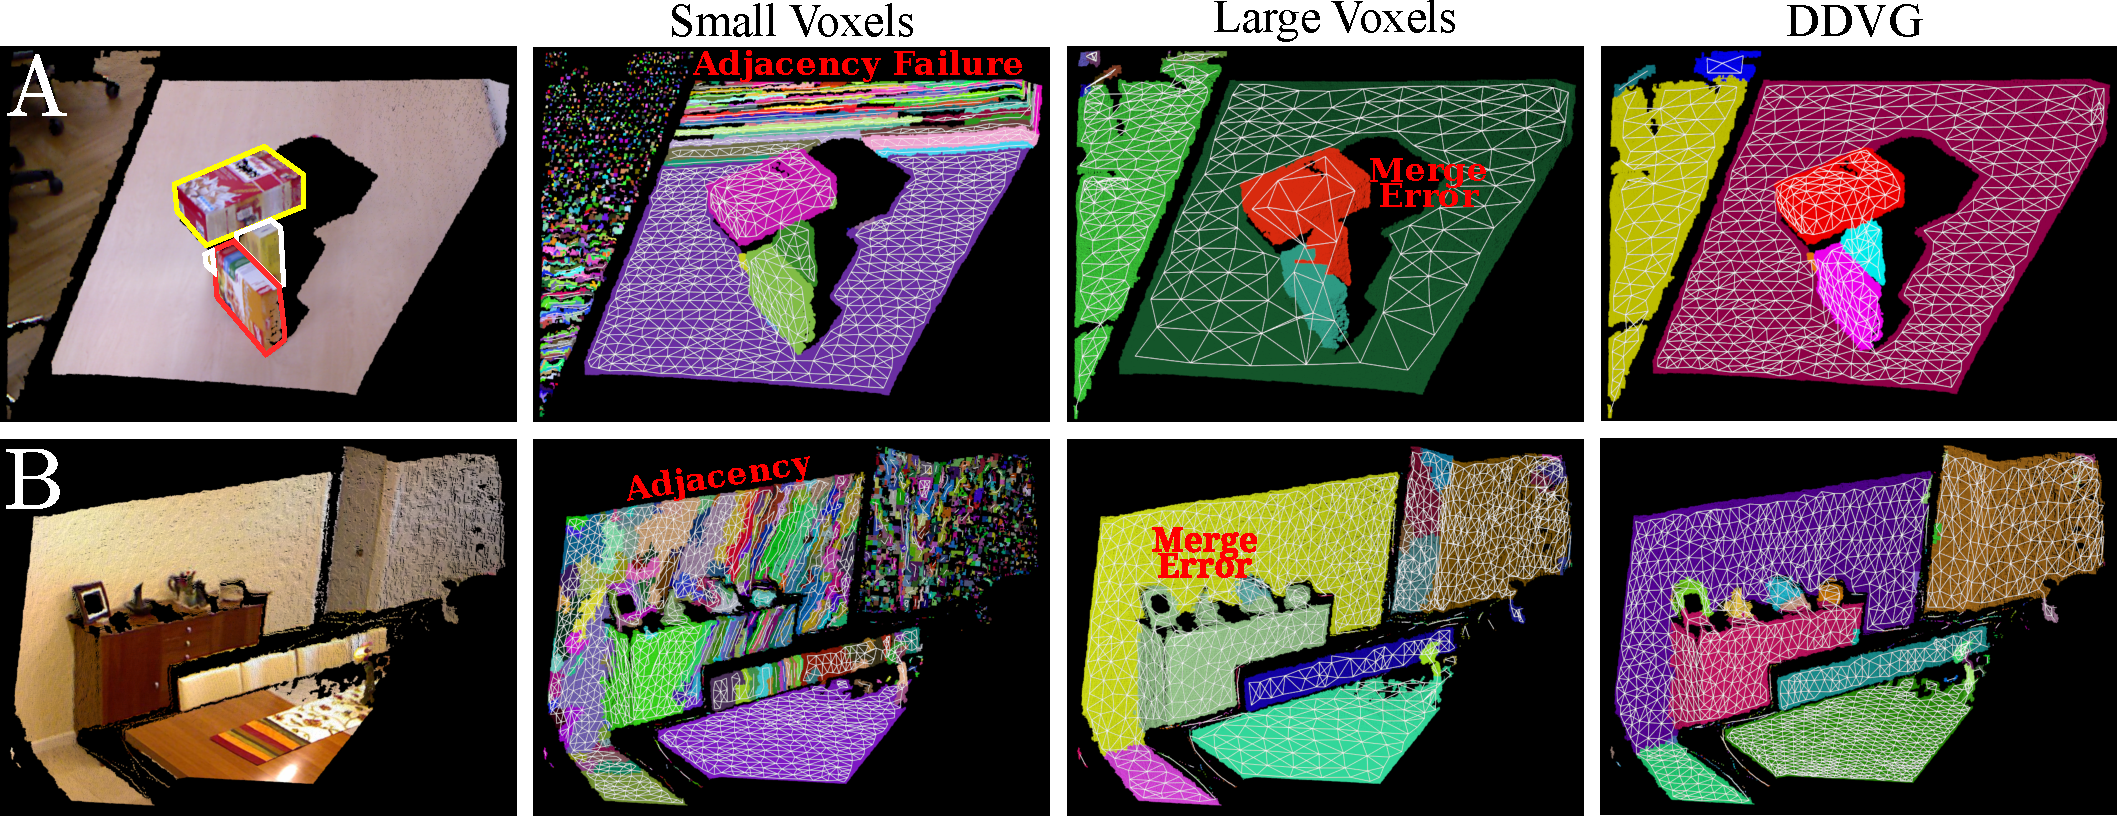
\includegraphics[width = \linewidth]{figures/CVPR2014/transform_results_v2}
\caption[Depth Adaptive Transform]{Two example point clouds \textbf{(A,B, left)} showing the need for the Depth Dependent Voxel Grid. For better visibility outlines have been drawn around the boxes in A. Using \textit{Small Voxels} objects close to the camera can be segmented, but adjacency breaks down as the depth increases and the point density decreases. Using \textit{Large Voxels} corrects the adjacency graph in the background, but leads to objects being merged in the foreground due to the coarse resolution. Using \textit{DDVG}, the scale of the voxels gradually increases with distance from the camera -- adapting to the increased noise level and lower point density -- consequently adjacency is maintained and the segmentation of scenes with large depth variance is possible using fixed parameters. Note, the flat rug on the table in B does not differ enough from the table's surface and cannot be segmented by any purely depth dependent method.}
\label{fig:quantization_transform}
\end{figure*}


\section{Experimental Results}

\label{sec:Evaluation}
In order to evaluate the quality of supervoxels generated by VCCS, we performed a quantitative comparison with three state-of-the-art superpixel methods using publicly available source code. 
We selected the two 2D techniques with the highest published performance from a recent review \cite{SLICCompared}: a graph based method, GCb10 \cite{SuperpixelsSupervoxels}\footnote{\url{http://www.csd.uwo.ca/~olga/Projects/superpixels.html}}, and a gradient ascent local clustering method, SLIC \cite{SLICCompared}\footnote{\url{http://ivrg.epfl.ch/supplementary_material/RK_SLICSuperpixels/index.html}}.
Additionally, we selected another method which uses depth images, DASP\cite{DASP}\footnote{\url{https://github.com/Danvil/dasp}}.
Examples of over-segmentations produced by the methods are given in Figure~\ref{fig:ExampleSegmentations}.
%------------------------------------------------------------------------
\begin{figure}[t]
\begin{center}
%\fbox{\rule{0pt}{2.4in} \rule{0.9\linewidth}{0pt}}
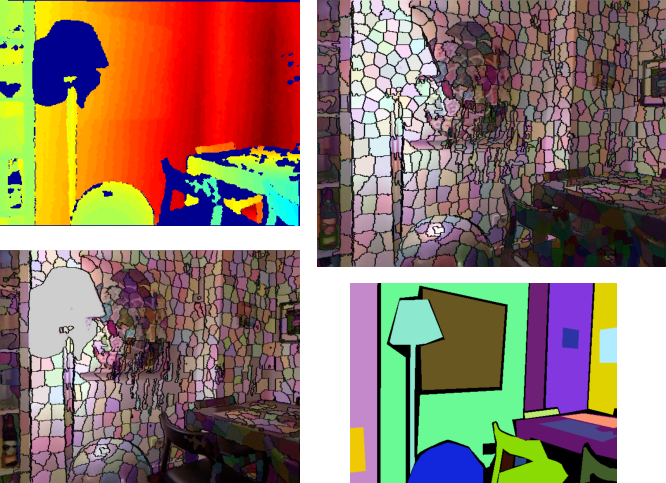
\includegraphics[width=0.9\linewidth]{figures/CVPR2013/BackTo2D.pdf}
\end{center}
   \caption[2D Hole Filling]{Example of hole-filling for images after returning from voxel-cloud to the projected image plane. Depth data, shown in the top left, has holes in it, shown as dark blue areas (here, due to the lamp interfering with the Kinect). The resulting supervoxels do not cover these holes as shown in the bottom left, since the cloud has no points in them. To generate a complete 2D segmentation, we fill these holes in using the SLIC algorithm, resulting in a complete segmentation, seen in the top right. The bottom right shows human annotated ground truth for the scene. }
\label{fig:ReturnToPlane}
\end{figure}
%------------------------------------------------------------------------

%------------------------------------------------------------------------
\begin{figure*}
\begin{center}
\includegraphics[width=1.01\linewidth]{figures/CVPR2013/Multiview.pdf}
\end{center}
   \caption[Supervoxels from Multiple Views]{Over-segmentation of a cloud from the RGB-D scenes dataset\cite{RGBDDataset}. The cloud is created by aligning 180 kinect frames, examples of which are seen on the left side. The resulting cloud has over 3 million points, which reduces to 450k points at ${R}_{voxel}=0.01m$ and 100k points with ${R}_{voxel}=0.02m$. Over-segmentation of these take 6 and 1.5 seconds, respectively (including voxelization).}
\label{fig:MultiViewCloud}
\end{figure*}
%------------------------------------------------------------------------

%------------------------------------------------------------------------
\begin{figure*}
\begin{center}
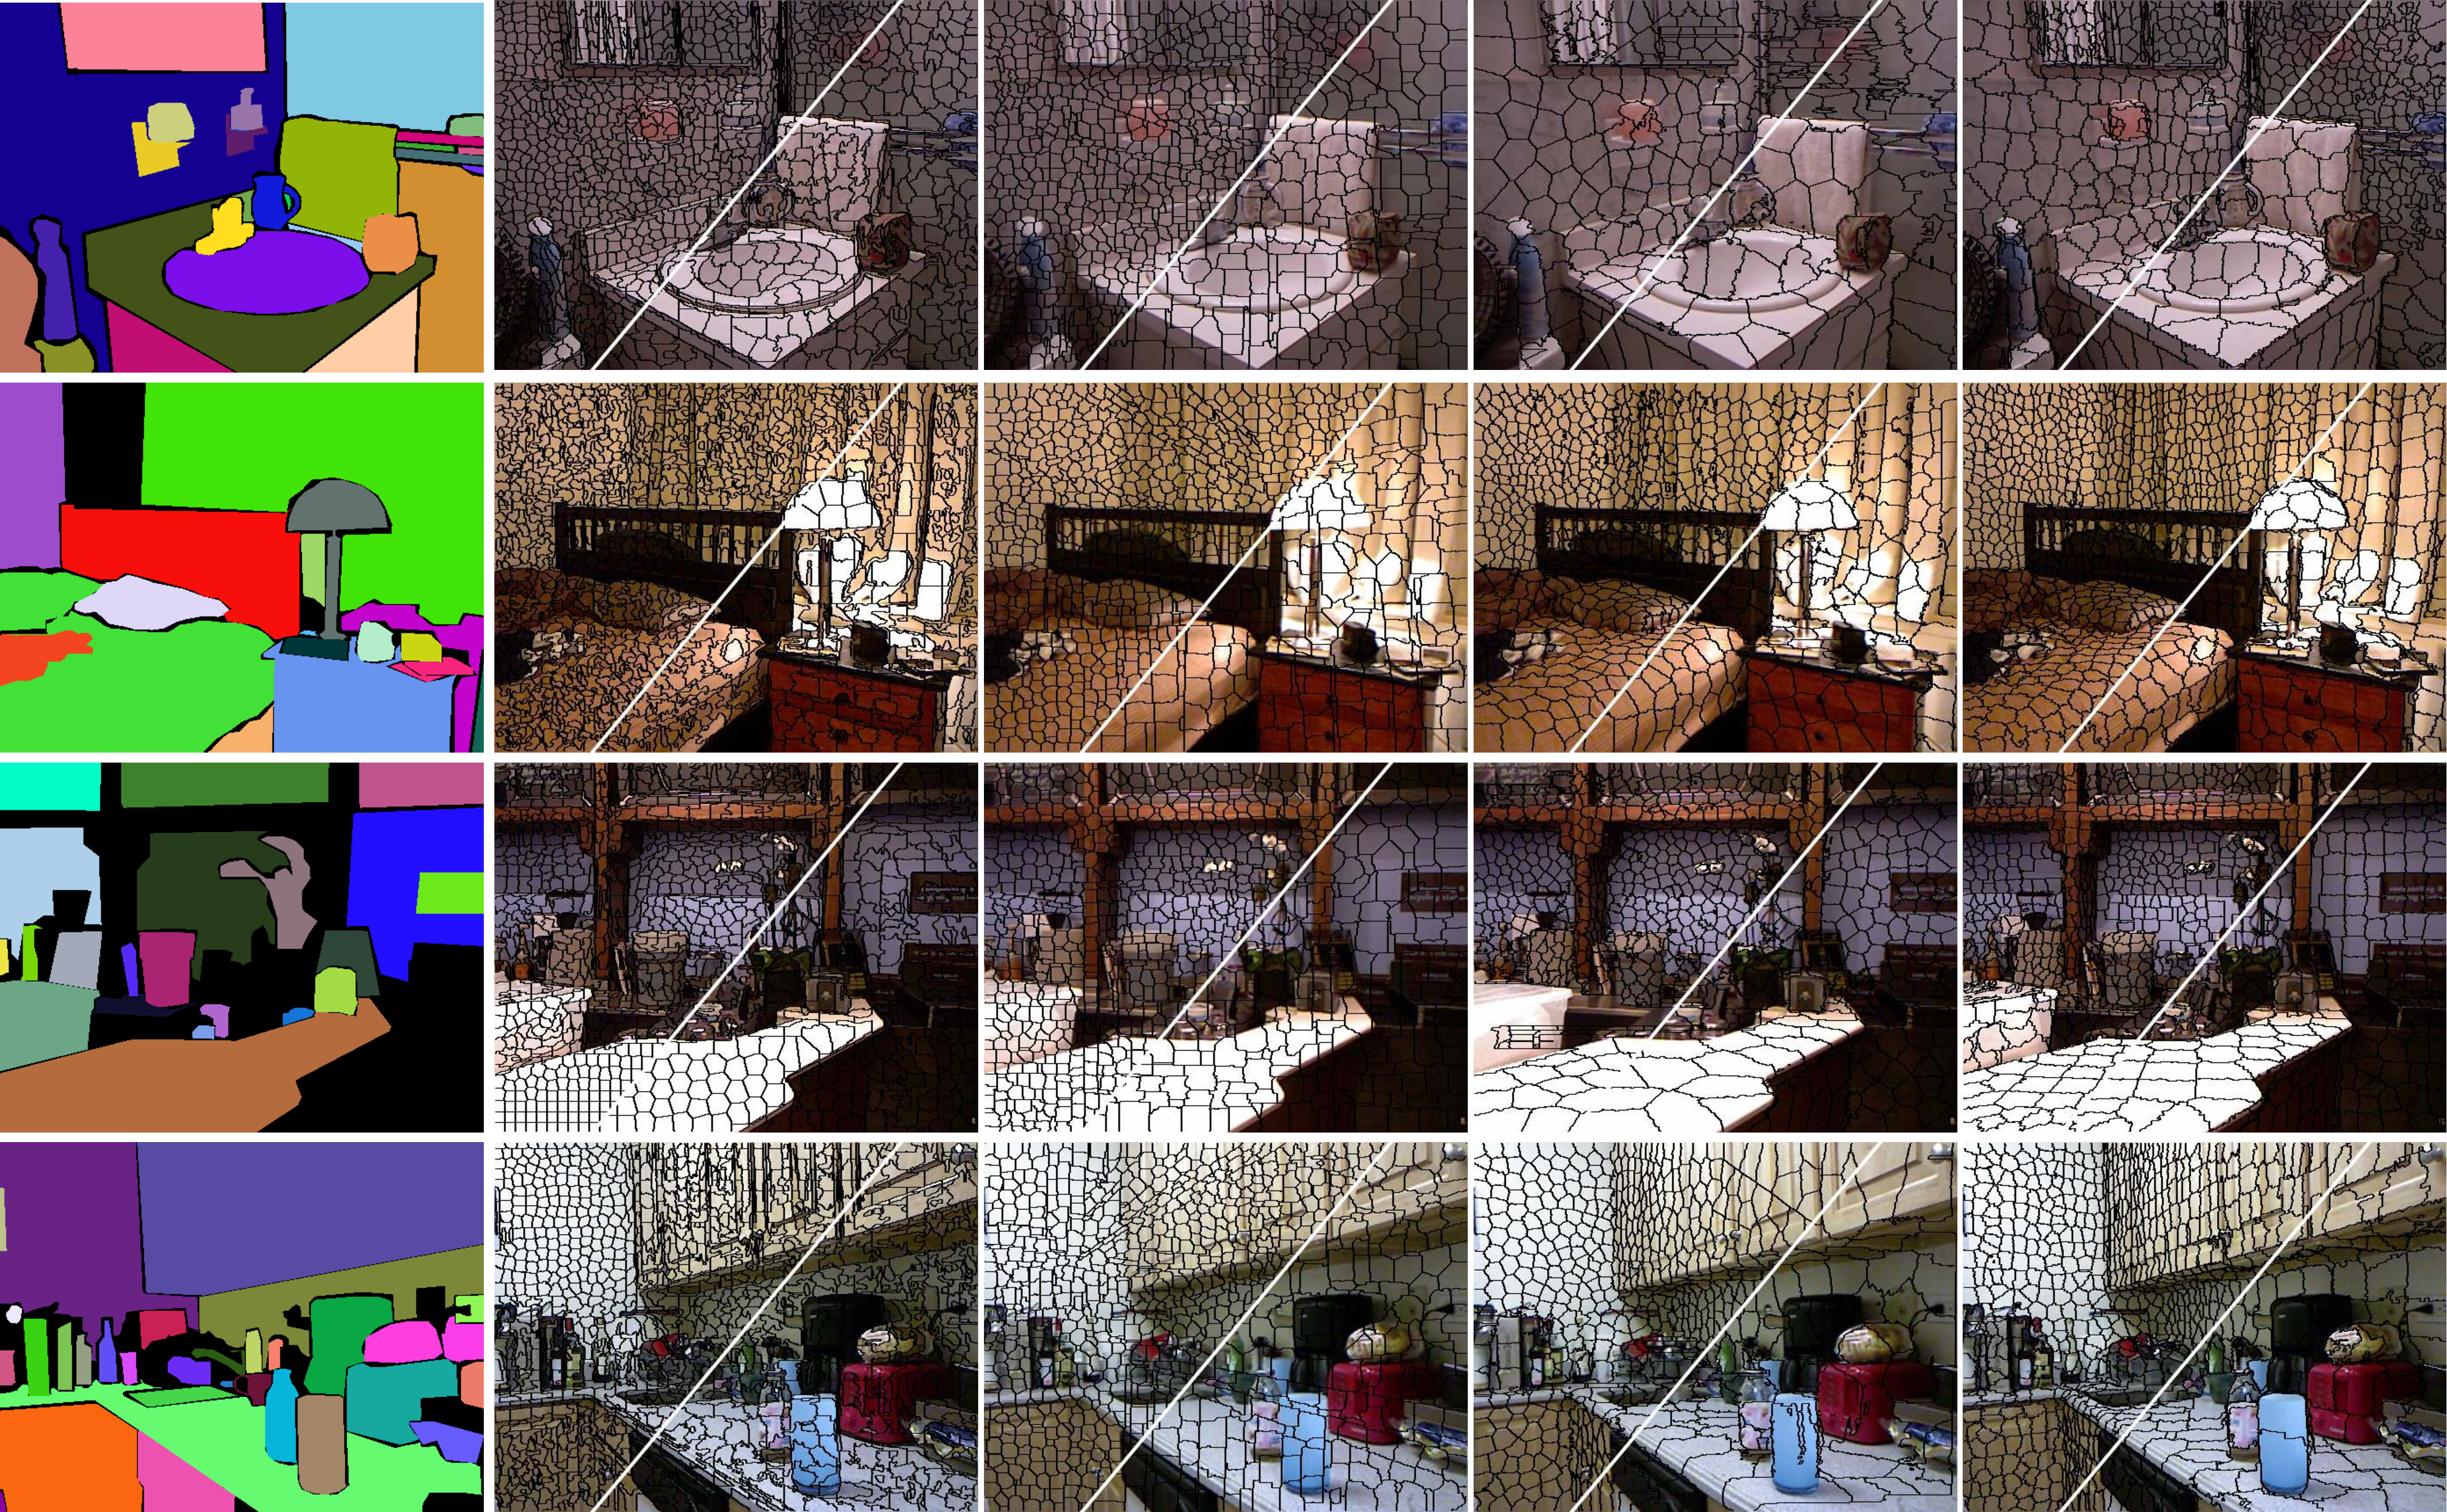
\includegraphics[width=1.01\linewidth]{figures/CVPR2013/Comparison_Segmentation_Small.pdf}
\end{center}
   \caption[Superpixel Comparison]{Examples of under-segmentation output. From left to right- ground truth annotation, SLIC, GCb10, DASP, and VCCS. Each is shown with two different superpixel densities.}
\label{fig:ExampleSegmentations}
\end{figure*}
%------------------------------------------------------------------------

\subsection{Dataset}
For testing, we used the recently created NYU Depth Dataset V2 semantic segmentation dataset of Silberman et al.\@ \cite{NYUDataset}\footnote{\url{http://cs.nyu.edu/~silberman/datasets/nyu_depth_v2.html}}. This contains 1449 pairs of aligned RGB and depth images, with human annotated densely labeled ground truth. The images were captured in diverse cluttered indoor scenes, and present many difficulties for segmentation algorithms such as varied illumination and many small similarly colored objects. Examples of typical scenes are shown in Figure~\ref{fig:ExampleSegmentations}.
%For further details on the dataset we refer the reader to the original work\cite{NYUDataset}. 

\subsection{Returning to the Projected Plane}
RGB+D sensors produce what is known as an organized point cloud- a cloud where every point corresponds to a pixel in the original RGB and depth images. When such a cloud is voxelized, it necessarily loses this correspondence, and becomes an unstructured cloud which no longer has any direct relationship back to the 2D projected plane. As such, in order to compare results with existing 2D methods we were forced to devise a scheme to apply supervoxel labels to the original image. 

To do this, we take every point in the original organized cloud and search for the nearest voxel in the voxelized representation. Unfortunately, since there are blank areas in the original depth image due to such factors as reflective surfaces, noise, and limited sensor range, this leaves us with some blank areas in the output labeled images. To overcome this, we fill in any large unlabeled areas using the SLIC algorithm. This is not a significant drawback, as the purpose of the algorithm is to form supervoxels in 3D space, not superpixels in the projected plane, and this hole-filling is only needed for comparison purposes. Additionally, the hole filling actually makes our results worse, since it does not consider depth, and therefore tends to bleed over some object boundaries that were correctly maintained in the supervoxel representation. An example of what the resulting segments look like before and after this procedure are shown in Figure~\ref{fig:ReturnToPlane}. 

%------------------------------------------------------------------------
\begin{figure}[t]
\begin{center}
%\includegraphics[width=0.8\linewidth,type=eps,ext=.eps,read=.eps]{Figures/boundary}
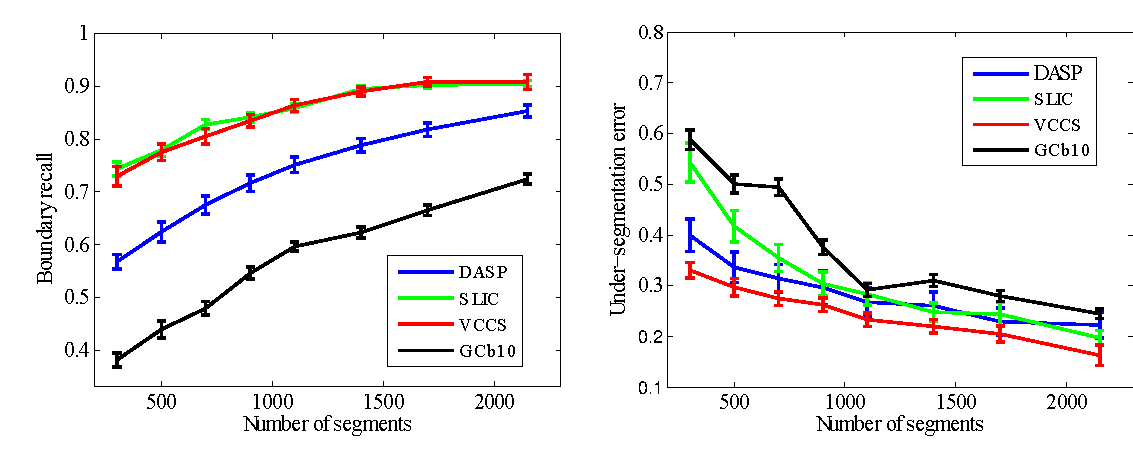
\includegraphics[width=0.95\linewidth]{figures/CVPR2013/Performance.pdf}
\end{center}
   \caption[Boundary Recall \& Undersegmentation Error]{Boundary recall and under-segmentation error for SLIC, GCb10, DASP, and VCCS.}
\label{fig:BoundaryRecall}
\label{fig:UndersegError}
\end{figure}
%------------------------------------------------------------------------

\subsection{Evaluation Metrics}
The most important property for superpixels is the ability to adhere to, and not cross, object boundaries. To measure this quantitatively, we have used two standard metrics for boundary adherence- boundary recall and under-segmentation error\cite{Turbopixels, SuperpixelsSupervoxels}. Boundary recall measures what fraction of the ground truth edges fall within at least two pixels of a superpixel boundary. High boundary recall indicates that the superpixels properly follow the edges of objects in the ground truth labeling. The results for boundary recall are given in Figure~\ref{fig:BoundaryRecall}. As can be seen, VCCS and SLIC have the best boundary recall performance, giving similar results as the number of superpixels in the segmentation varies. 

Under-segmentation error measures the amount of leakage across object boundaries. For a ground truth segmentation with regions $g_1,...,g_M$, and the set of superpixels from an over-segmentation, $s_1,...s_K$, under-segmentation error is defined as 
\begin{equation}
\label{eqn:UndersegError}
{E}_{useg}=\frac{1}{N} \left[ \sum_{i=1}^{M}{\left(\sum_{s_j \mid s_j \cap g_i}{|s_j|}\right)-N} \right],
\end{equation}
where $s_j \mid s_j \cap g_i$ is the set of superpixels required to cover a ground truth label $g_i$, and $N$ is the number of labeled ground truth pixels. A lower value means that less superpixels violated ground truth borders by crossing over them. Figure~\ref{fig:UndersegError} compares the four algorithms, giving under-segmentation error for increasing superpixel counts. VCCS outperforms existing methods for all superpixel densities. 

\subsection{Time Performance}
As superpixels are used as a preprocessing step to reduce the complexity of segmentation, they should be computationally efficient so that they do not negatively impact overall performance. To quantify segmentation speed, we measured the time required for the methods on images of increasing size (for the 2D methods) and increasing number of voxels (for VCCS). All measurements were recorded on an Intel Core i7 3.2Ghz processor, and are shown in Figure~\ref{fig:SegmentationSpeed}. VCCS shows performance competitive with SLIC and DASP (the two fastest superpixel methods in the literature) for voxel clouds of sizes which are typical for Kinect data at ${R}_{voxel}=0.008m$ (20-40k voxels). It should be noted that only VCCS takes advantage of multi-threading (for octree, kd-tree, and FPFH computation), as there are no publicly available multi-threaded implementations of the other algorithms.  

%------------------------------------------------------------------------
\begin{figure}[t]
\begin{center}
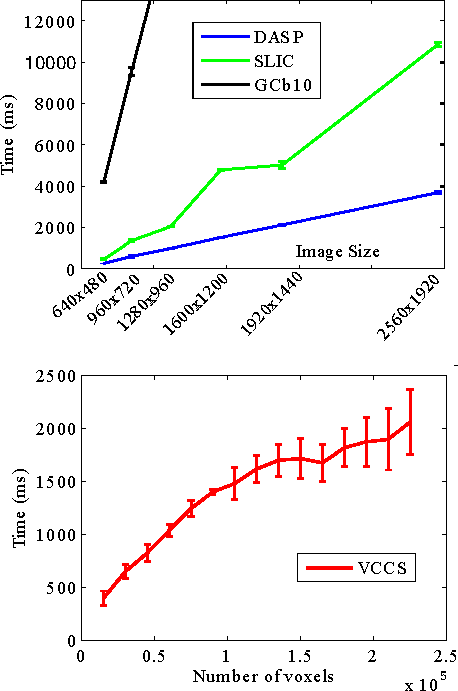
\includegraphics[width=0.95\linewidth]{figures/CVPR2013/Speed.pdf}
\end{center}
   \caption[Segmentation Speed]{Speed of segmentation for increasing image size and number of voxels. Use of GCb10 rapidly becomes unfeasible for larger image sizes, and so we do not adjust the axes to show its run-time. The variation seen in VCCS run-time is due to dependence on other factors, such as ${R}_{seed}$ and overall amount of connectivity in the adjacency graphs.}
\label{fig:SegmentationSpeed}
\end{figure}
%------------------------------------------------------------------------

\section{Sequential Update of Perceptual Model}
Adding newly observed points to an existing supervoxel octree is accomplished through a three stage process. First, we must insert the points into the octree, and initialize new leaves for them if they did not exist previously. This results in an octree where leaves fall into three possible categories (illustrated in Fig.~\ref{fig:VoxelVisibility}; they are either new, observed, or unobserved in the most recent observation. Handling of new leaves is straightforward; we simply calculate adjacency relations to existing leaves and flag them as unlabeled. 
\begin{figure}[tb]
  \centering
  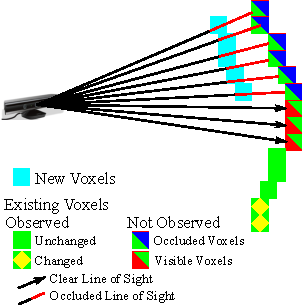
\includegraphics[scale=1.2]{figures/IROS2013/VoxelVisibility.pdf}
  \caption[Voxel Visibility]{Categorization of voxels based on new frame of data. Voxels fall into three categories, they are either new, observed or not observed in the frame. Furthermore, observed voxels can either have changed or remained the same, while voxels not observed in the frame are either occluded or no longer exist (in which case they should be deleted).}
  \label{fig:VoxelVisibility}
\end{figure}

To determine whether a leaf which existed previously has changed, we test the distance between the centroid of the points falling within its voxel (from the new frame) and its previous centroid. This is done in the same feature space used for growing the supervoxels, that is, we test whether the normal, color, and spatial location have varied more than a threshold value. This threshold is set to a relatively low constant value so that it favors false-positives (finding change when there was none), as they do not impact the tracking performance of the algorithm, but only have a slight effect on its run-time.  If a leaf is found to have changed, we remove its previous labeling. We also perform a global check to see if more than half of a supervoxels support has changed; if so, we completely remove the supervoxels label from all of its constituent voxels. 

Finally, we must consider how to handle leaves which were not observed in the inserted point cloud. Rather than simply prune them, we first check if it was possible to observe them from the viewpoint of the sensor which generated the input cloud. This occlusion check can be accomplished efficiently using the octree by determining if any voxels exist between unobserved leaves and the sensor viewpoint. If a clear line of sight exists from the leaf to the camera, it can safely be deleted. Conversely, if the path is obstructed, we "freeze" the leaf, meaning that it will remain constant until it is either observed or passes the line of sight test in a future frame (in which case, it can be safely deleted). This occlusion testing means that tracking of occluded objects is trivial, as occluded voxels remain in the observations which are used for tracking.

Once the octree voxels have been updated, we then proceed to update the supervoxels as before. That is, first we generate new seeds in regions of large unlabeled voxels, and then conduct the iterative region growing. This results in new supervoxels in regions which are new or changing, while leaving supervoxels in static and occluded regions unchanged. This reduces the tracking and segmentation problem to finding the best joint association of these new supervoxels with those from the prior time-step.

\section{Discussion}


%% Requires fltpage2 package
%%
% \begin{FPfigure}
% \includegraphics[width=\textwidth]{figures/fullpage}
% \caption[Short figure name.]{This is a full page figure using the FPfigure command. It takes up the whole page and the caption appears on the preceding page. Its useful for large figures. Harvard's rules about full page figures are tricky, but you don't have to worry about it because we took care of it for you. For example, the full figure is supposed to have a title in the same style as the caption but without the actual caption. The caption is supposed to appear alone on the preceding page with no other text. You do't have to worry about any of that. We have modified the fltpage package to make it work. This is a lengthy caption and it clearly would not fit on the same page as the figure. Note that you should only use the FPfigure command in instances where the figure really is too large. If the figure is small enough to fit by the caption than it does not produce the desired effect. Good luck with your thesis. I have to keep writing this to make the caption really long. LaTex is a lot of fun. You will enjoy working with it. Good luck on your post doctoral life! I am looking forward to mine. \label{fig:myFullPageFigure}}
% \end{FPfigure}
% \afterpage{\clearpage}
